\section{Setup} 
\subsection{Requirements}
In this section all of the requirements needed are described.
\subsubsection{Browser}
\textit{Soldino} is accessible through a web interface. The currently most recent versions of the following broswers are supported:
\begin{itemize}
	\item \textbf{Mozilla Firefox}: version 64 or later;
	\item \textbf{Google Chrome}: version 71 or later.
\end{itemize}

\subsubsection{Tools}
The following tools are needed:
\begin{itemize}
	\item \textbf{Git}: a famous control version system: \textit{Soldino}'s repository is hosted on GitHub;
	\item \textbf{Node.js}: a framework needed for installing dependencies;
	\item \textbf{Truffle}: needed to write and deploy contracts with ease;
	\item \textbf{Ganache}: needed to put up a local Ethereum network and check transactions in it;
	\item \textbf{Metamask}: a browser plugin used as a virtual wallet;
	\item \textbf{Surge.sh}: a web platform chosen for hosting the website interface of Soldino.
\end{itemize}

\subsubsection{Dependencies}
Soldino depends on many different packages, some for use and others for development.\\
All these dependencies can be found in the file \texttt{package.json} which is in the root folder of the project.\\
The packages required to execute the software \textit{Soldino} are listed below.\\

\renewcommand{\arraystretch}{1.5}
\rowcolors{2}{pari}{dispari}
\begin{longtable}{ 
		>{\centering}p{0.4\textwidth} 
		>{\centering}p{0.4\textwidth}
	}
	\caption{Packages required for software usage}\\
	\rowcolorhead
	\textbf{\color{white}Software} & 
	\textbf{\color{white}Version}
	\tabularnewline  
	\endhead	
	
	% voci prese da package.json, repo "Soldino-PoC, ramo "develop"


	react-text-mask & $\geq$5.4.4
	\tabularnewline
	commondir &$\geq$1.0.1
	\tabularnewline
	history &$\geq$4.7.2
	\tabularnewline
	prop-types &$\geq$15.7.2\tabularnewline
	react &$\geq$16.8.3\tabularnewline
	react-dom &$\geq$16.8.3\tabularnewline
	react-number-format &$\geq$4.0.6\tabularnewline
	react-redux &$\geq$6.0.1\tabularnewline
	react-router &$\geq$4.3.1\tabularnewline
	react-router-dom &$\geq$4.3.1\tabularnewline
	react-router-redux &$\geq$4.0.8\tabularnewline
	react-scripts &$\geq$2.1.8\tabularnewline
	redux &$\geq$4.0.1\tabularnewline
	redux-thunk &$\geq$2.3.0\tabularnewline
	web3 & 1.0.0-beta.37\tabularnewline
	
\end{longtable}

Other packages, listed below, are required for the development.
\renewcommand{\arraystretch}{1.5}
\rowcolors{2}{pari}{dispari}
\begin{longtable}{ 
		>{\centering}p{0.4\textwidth} 
		>{\centering}p{0.4\textwidth}
	}
	\caption{Packages required for development}\\
	\rowcolorhead
	\textbf{\color{white}Software} & 
	\textbf{\color{white}Version}
	\tabularnewline  
	\endhead	
	
	% voci prese da package.json, repo "Soldino-PoC, ramo "develop"
	eslint & 5.12.0\tabularnewline
	eslint-config-airbnb &$\geq$17.1.0\tabularnewline
	eslint-loader & $\geq$2.1.2\tabularnewline
	eslint-plugin-import & $\geq$2.16.0\tabularnewline
	eslint-plugin-jsx-a11y & $\geq$6.2.1\tabularnewline
	pre-commit & $\geq$1.2.2\tabularnewline
	truffle-contract & $\geq$4.0.6
	
\end{longtable}

\subsection{Installing}
\subsubsection{Browser}
The first thing is to have your browser installed. You can get the latest Chrome version  \href{https://www.google.com/chrome/}{here} or the latest Firefox version \href{https://www.mozilla.org/en-US/firefox/new/}{here}\\

\subsubsection{Git}
You should type this script in the shell for installing Git packet: \texttt{sudo apt install git}.

\subsubsection{Node}
For installing Node.js you have to digit in the shell the following commands:
\begin{enumerate}
	\item \texttt{curl -sL https://deb.nodesource.com/setup\_11.x | sudo -E bash -}
	\item \texttt{sudo apt install -y nodejs}
	\item check that \texttt{node} have been installed correctly with \texttt{node -v}.
\end{enumerate}
There is no need to install npm separately, since it is automatically installed with Node.

\subsubsection{Truffle}
You should check you have the truffle requirements:
\begin{itemize}
	\item an OS among Linux, Windows and MacOS (prefer Linux);
	\item NodeJS v8.9.4 or later (we picked version 11);
	\item Node Package Manager (npm).
\end{itemize}
then you can install Truffle by running the command: \texttt{npm install -g truffle}

\subsubsection{Ganache}
There are three step to install Ganache:
\begin{enumerate}
	\item you can download the Ganache executable at this \href{https://truffleframework.com/ganache}{link}, clicking on the download button;
	\item if you have a Linux operating system, you have to give the permissions to make the Ganache file executable. This can be done with the command \\\texttt{chmod +x path-of-the-appimage/name-of-downloaded-file.AppImage};
\end{enumerate}

\subsubsection{MetaMask}
You can add it to your browser in this way:
\begin{itemize}
	\item Chrome:  \href{https://chrome.google.com/webstore/search/metamask?hl=it}{https://chrome.google.com/webstore/search/metamask?hl=it};
	\item Firefox: \href{https://addons.mozilla.org/it/firefox/addon/ether-metamask/?src=search}{https://addons.mozilla.org/it/firefox/addon/ether-metamask/?src=search}.
\end{itemize}


\subsubsection{Surge}
You have to install Surge by executing the shell command: \texttt{npm install -g surge}.


\subsection{Configuration}
This section shows how to configure your work environment, so that it's the same as ours, in order to minimize the number and entity of troubles you will occur in.\\
Make sure to configure the tools in order. In particular, Truffle requires that Ganache is opened and is configured to execute successfully.
% clona la repo; apri truffle, apri ganache, apri browser con metamask, setta
\subsubsection{Cloning the repo}
You have to clone the \textit{Soldino} repository on GitHub: open the shell, move to the directory where you want Soldino to be, then use \texttt{git clone https://github.com/8LabSolutions/Soldino-PoC} and then use \texttt{git checkout final
}.  

\subsubsection{Ganache}
You have to go to the folder where you've put Ganache, and open it with double click.
\begin{figure}
	\centering
	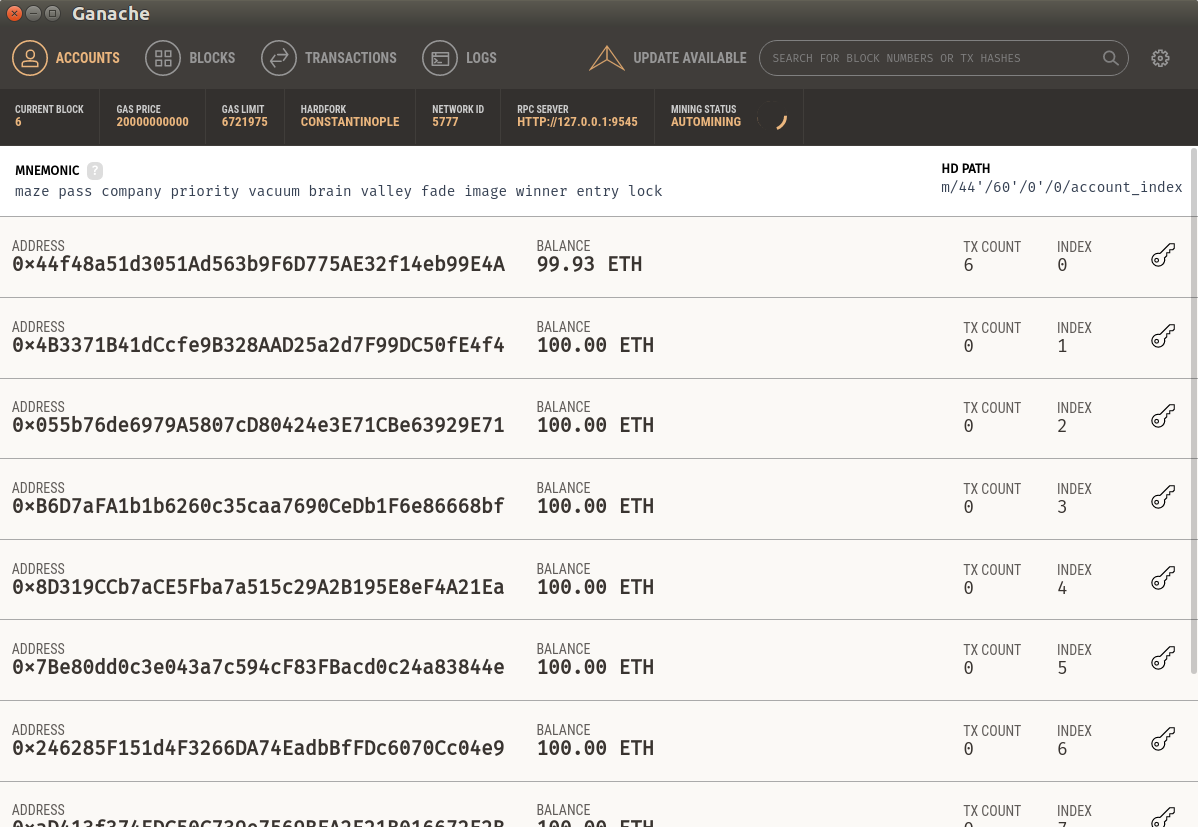
\includegraphics[scale=0.25]{res/images/ganache-ui.png}
	\caption{Ganache UI: from top to bottom you can see the menu bar, the current configuration, the mnemonic, and the interface of the selected menu option}
\end{figure}
Then you have to click on the cogwheel at the top left corner to access Ganache settings and make sure you've matched the following settings (most of which are defined in \texttt{truffle-config.js}) on each respective window:
\begin{itemize}
	\item Server:
	\begin{itemize}
		\item hostname: \texttt{127.0.0.1};
		\item port number: \texttt{9545};
		\item network id: any (you can keep the default one).
	\end{itemize}
	\item Account \& keys:
	\begin{itemize}
		\item nothing to configure here, but you should have a look at the \textbf{mnemonic}: it will help you later.
	\end{itemize}
\end{itemize}

\subsubsection{Truffle}
The configuration of Truffle is defined in the file \texttt{truffle-config.js} in the root directory of \textit{Soldino}.
On your shell type the following shell commands:
\begin{itemize}
	\item \texttt{truffle console}\\
	opens the truffle environment in the shell under the configuration defined in truffle-config.js. From now on, every command is executed in the truffle environment, from which you can exit double typing \texttt{ctrl + C}.
	\item \texttt{compile}\\
	to compile the contracts: these are compiled in in a .json format (which enables interaction with the frontend) and put into the folder defined in \texttt{truffle-config.js} at \texttt{contracts\_build\_directory} (in our case the location is \texttt{./src/contracts\_build})
	\item \texttt{migrate -{}-network development}\\
	puts the contracts runnning on the blockchain. 
\end{itemize}

\subsubsection{MetaMask}
It's necessary to create an account.
\begin{itemize}
	\item open MetaMask on your browser
	\item select get started
	\item select import wallet
	\item use the seed frase (AKA the mnemonic) copy pasting the one \item from ganache and put your password
\end{itemize}
Now your account is up and synchronized with Ganache.
Now you have to connect the wallet to Ganache network. Ganache settings are exposed in the Ganache UI just above the mnemonic.
Let's synchronize MetaMask to the same network. On the top right corner there is a drop-down menu to select the network. Select \texttt{Custom RPC} to set your own local network.\\
You are now in the MetaMask advanced settings screen. In the field \texttt{Net Network} click on \texttt{Show Advanced Options} to open the form, then insert these data:
\begin{enumerate}
	\item \textbf{New RPC URL}: http://127.0.0.1:9545 (the port number matches the one in truffle-config.js);
	\item \textbf{Nickname}: the name you wanna give to your network;
	\item \textbf{save} when you're done.
\end{enumerate}
MetaMask is now connected to Ganache.\\

To enable transactions on your local test network, you can find free ether for testing networks on this site: \href{https://faucet.metamask.io/}{https://faucet.metamask.io/}.

% PUT CUBIT TO METAMASK

\subsection{Running}
Now that you have all the required software installed and configured, it's time to get it up running.\\
All you have to do is moving to the root directory of Soldino and prompt
\begin{itemize}
	\item[]\texttt{npm run start}
\end{itemize}
This will open the website on your browser at the address \texttt{http://127.0.0.1:3000} and allow you to explore it. 


%\subsection{Deploying}
%This part shows you how to deploy contracts with Truffle and have them up running on Soldino.
%
% qua c'è surge, il deploy su ropsten, etc. VAnno cambiati alcuni file nei parametri di configurazione
% 